\chapter{Conclusion}
\label{cha:conclusion}

This dissertation investigated the design, implementation, and evaluation of a serious game framework for sustainability called Makahiki, and a stakeholder experience based assessment me-thod (SGSEAM) for assessing serious game frameworks. This chapter summarizes the results of the research, the contributions of the research, and possible future directions.

\section{Research Summary}

This research investigates the information technology infrastructure that can support effective and efficient development of serious games for sustainability. The research includes the development of an innovative serious game framework for sustainability called Makahiki, and an assessment method called SGSEAM to access the strengths and weaknesses of the IT infrastructure for serious games for sustainability with regarding the stakeholder's perspective.

The motivation of Makahiki is to provide a low cost and better alternative to the IT infrastructure that enables the creation and managing of collegiate sustainability competitions from different organizations. The design of Makahiki is inspired by the current research in game design in the context of both serious games and gamification. 

I led an effort over the past years to design and implement the Makahiki framework. Makahiki is an open source serious game framework for sustainability, which includes a variety of common services for developing sustainability games including authentication; game mechanics such as leaderboards, points, and badges; a variety of built-in games and content focused in sustainability, a responsive user interface, cloud-based deployment, and the ability to customize to the needs of individual organizations.

Makahiki had been used to create and manage seven (7) real-world sustainability games by four (4) organizations, in different environments and with different requirements. The instances are: 
\begin{enumerate}
\item the Kukui Cup energy challenges at the University of Hawaii at Manoa in 2011, 2012 and 2014 (UHM).
\item the HPU Kukui Cup energy challenges at the Hawaii Pacific University in 2012 and 2013 (HPU).
\item the East West Center energy and water challenge in 2012 (EWC).
\item the Kukui Cup educational challenge at the Holy Nativity School in 2013 (HNS). 
\end{enumerate}

The major differences between these instances are:
\begin{itemize}
\item Resource collection: UHM and HPU used different metering infrastructure for automatically energy data collection. EWC collected their resource data manually, and HNS did not have energy data at all. 
\item UHM and HPU challenges involved only energy consumption data, the EWC challenge involved both energy and water consumption data. 
\item UHM and HPU provided authentication services using CAS and LDAP, while EWC used both CAS and the built-in Django internal  authentication, and HNS used only the internal authentication
\item User interfaces were customized to ``brand'' each challenge with the logo, thematic elements, and the education contents of the sponsoring organizations.
\item HPU instances were hosted in its local infrastructure, while UHM, EWC and HNS were hosted in the Heroku PaaS cloud.
\end{itemize}

I assisted the HPU system admin to install their instances in HPU's infrastructure, and integrate with HPU's LDAP and email server, which were found to be the most difficult tasks in HPU's installation. I also deployed the UHM, EWC and HNS instances to the Heroku cloud and actively managed these cloud instances. 

While these real world Makahiki instance provides initial evidence regarding the ability of the Makahiki framework to support sustainability games in different environments, a more rigorous evaluation of Makahiki would yield better quality insight. During my literature search, I have not found any research in the area of formal evaluation for serious game {\em \bf framework}, although there exists several assessment methods for serious games and for general purpose evaluation such as system usability. 

The design of SGSEAM is to provide an assessment method for the particular needs of assessing a serious game framework. SGSEAM describes a stakeholder perspective based method to provide detailed insight into the strengths and weaknesses of a serious game framework. It identifies the major stakeholders whose experiences affect a serious game framework as a software infrastructure are players, system admins, game designers, game managers and game developers. For each stakeholder, multiple assessment approaches can be used, depending on the resources available. The more approaches applied, the higher one's confidence in the accuracy of the assessment results.

In my research, I applied SGSEAM to Makahiki in order to gain better insight into its strengths and weaknesses as a serious game framework. The {\em in-vivo} assessment approaches of pre-post effectiveness study, in-game surveys and post-hoc interviews were applied to the real-world Kukui Cup challenges created by the Makahiki framework, while the {\em in-vitro} assessment approaches of in-lab study used the UHM ICS691 serious game course to assess the experiences in game installation, game design and game development. 

The application of SGSEAM to Makahiki had effectively identified several strengths and weaknesses of the Makahiki as the serious game framework for sustainability, and produced the improvement action report to Makahiki developer to improve the framework. SGSEAM revealed that Makahiki is capable in enabling organizations to create effective and engaging serious games for sustainability. It also revealed the major weaknesses of Makahiki are difficulty in developing new enhancements,  difficulty in integrating external LDAP and email server, and the lack of WYSIWYG content authoring tool.

\section{Contributions}

My research has generated several contributions, including: 1) Makahiki: A serious game framework for sustainability; 2) Real-world use of Makahiki;  3) Insights into managing a cloud based serious game; 4) SGSEAM: a serious game framework assessment method; 5) Strengths and weaknesses of Makahiki.

\subsection{Makahiki: A serious game framework for sustainability}

The Makahiki framework described in \autoref{cha:makahiki-design} contributes to the field of serious games
and sustainability. Makahiki creates a unique type of serious games that combine
both data on resource consumption and game content related to sustainability, represents an innovation in the area of serious game and sustainability education. 

Makahiki enables different organizations to easily create customized serious games in the context of sustainability education and behavioral change. As a framework, it includes the following features: 1) the ability to tailor system functionality to support the requirements of different organizations. 2) the ability to support sustainable resource challenges such as water, food, and waste in addition to energy. 3) the ability to extend the framework with new game and modules to support different requirements. 4) the use of HTML5/CSS3 ``responsive'' design techniques for support of laptop, tablet, and smart phone interfaces. 5) real-time game analytics to help assess the impact of game mechanics during challenges. 6) support for PaaS (Platform as a Service) facilities such as Heroku. This enables organizations to create and deploy challenges without obtaining physical hardware and its requisite IT support.

Makahiki is an open source system hosted on GitHub \cite{makahiki2} with less restricted MIT open source license. It  consists of over 37,000 lines python source code, 14,000 line of html code,  17,000 line of javascript code, and 42,000 line of documentation. 

\subsection{Real-world use of Makahiki}

Makahiki contributed to the creation and running of seven (7) real-world sustainability games by four (4) organizations. These game instances engaged the over 3,770 total students from the 4 educational institutes (University of Hawaii at Manoa, Hawaii Pacific University, East West Center and Holy Nativity School). Through the game interface, Students learned about the sustainability online and act in the reality to conserve energy and water consumption and other sustainability related behaviors. The in-game survey results from the multiple UHM instances indicate that the games had positive impacts on their energy literacy, self-reported sustainability awareness and self-reported behavior changes. Both the UHM and HPU instances achieved about 30\% player participation rate, which may lead to impacts to the community around the participants. The engagement metrics based on the game data from 2011 and 2012 UHM instances also indicates high level of player engagement during the 3-4 weeks period.

These games were created in various configurations and hosting environments. The successful creation of these serious game instances provides evidence that Makahiki can be successfully tailored to the needs of different organizations.

%% TODO Insights into creating and running several serious games in real-world

\subsection{Insights into managing a cloud based serious game}

I deployed and managed the EWC, HNS and the 2012, 2014 UHM instances in the Heroku PaaS cloud infrastructure. Although there are some hosting associated costs, it was considered cost effective in these real world instances by eliminating the needs to find and maintain a local server infrastructure. It also provided the capability of infrastructure scaling down and up when needed. In the case of EWC and HNS, because these two organizations did not have enough capacity and resources to use the local hosting option, they were  sponsored the Kukui Cup research grants to host their instances in the Heroku cloud infrastructure with us providing technical supports. 

As discussed in \autoref{section:cloud-hosting}, the cost for EWC and HNS instances are inexpensive. The Makahiki's support for hosting the game in the cloud lowered the barriers for these organizations to run this kind of serious games to achieve their educational and sustainability goal.

Hosting and managing the two UHM instances in the cloud provided interesting experiences with cloud based serious game. A performance test was done to estimate the appropriate initial provision to the game instance. During the game, the cloud monitoring service was used to monitor the performance and the utilization of resources. Depending on the usage demand during the game, the cloud infrastructure resource were re-allocate without stopping the game. 

The successfully use of Makahiki in the Heroku cloud platform provided a good alternative to organizations such as EWC and HNS who have less technology capacities. It also provides greater flexibility in infrastructure scaling up and down depending on the usage demand. In the context of serious games, which are often running for a period of time and have various usage demand throughout the game period, using the cloud infrastructure is a good consideration.

\subsection{SGSEAM: A serious game framework assessment method}

The SGSEAM described in \autoref{cha:sgseam-design} contributes to the emerging field of serious game framework evaluation research. SGSEAM describes a method for assessing serious game frameworks from the stakeholder experience perspective. The goal of SGSEAM is to identify (a) major strengths of a serious game framework, which aids the community by indicating features of the framework to emulate, and
(b) major shortcomings of the framework, which aids the community by indicating features to avoid.
The benefits of SGSEAM assessment are for the developers of serious game frameworks 
to learn and improve from the findings of the assessment.

SGSEAM identifies the major stakeholders of a serious game affected the software framework are players, system admins, game designers, game managers and game developers. For each serious game stakeholder, SGSEAM proposes several assessment approaches such as pre-post test, in-game surveys, post-hoc interviews, and in-lab experiments.

\subsection{Strengths and weaknesses of Makahiki}

The application of SGSEAM to Makahiki identified several strengths and weaknesses of  Makahiki as the serious game framework for sustainability. The strength and weakness report and improvement action report deliverable of this research provides valuable inputs to Makahiki developers for improving the framework, thus benefits the community and organizations that use Makahiki as a tool for sustainability education and behavior change. The strengths and weaknesses also help the serious game framework design community to learn from the strengths in Makahiki, and to avoid the shortcomings of Makahiki discovered in the SGSEAM assessment. 

\subsection{Wattdepot: A system for energy data management and analysis}

Wattdepot \cite{csdl2-10-05} is Java-based open source system to collect, store, analyze, and display energy data. It is used by Makahiki to provide real-time energy feedback and visualization to players participated in the energy challenges. Wattdepot version 2 was developed over a period of two years and had been used in the real world Makahiki game instances for UHM and HPU.  

Working with the primary developer, Robert Brewer, my role in the Wattdepot version 2 project was providing use case requirements from Makahiki, internal testing, and visualization development. working with the primary developer Carleton Moore, I participated in to the design of the new Wattdepot version 3, implemented the Google visualization API and the javascript API, and provided performance tuning for the Wattdepot database.

\section{Future Directions}

There are a variety of directions that can be pursued once this research is complete. This section discusses a variety of areas for future research.

\subsection{Applying SGSEAM to other serious game frameworks}
\label{future:other-framework}

The design of SGSEAM creates a research question of what are the strengths and weaknesses of this assessment method. To better answer this question, SGSEAM should be applied to another serious game development environment. BuildingOS\cite{building-dashboard} by Lucid Design Group is such a serious game framework that is suitable for SGSEAM evaluation. Our research lab had made the effort to contact Lucid Design group for the collaboration. I created the assessment plan (\autoref{app:sgseam-lucid-guide}) for them which hope to minimize the effort spent from their side. But due to the workload of the Lucid design group, the collaboration did not continue. It is understandable that Lucid design group, as a newly found startup company, has other urgent endeavors to pursue. Looking for another suitable serious game framework to apply SGSEAM assessment is still an ongoing research direction.

\subsection{Community or Consortium to expand the content and game library}

In order to provide more engaging experience to players, there are needs to expand the game content and even new type of games. They are not east tasks to maintaining an active existing game content while keeping adding new content to reflect contemporary issues. New type of games such as 3D simulation game would provide more fun and possible better engagement, but also requires large efforts to create such games. Building a community or consortium to expand content and game library for Makahiki could be a more sustainable approach. 

This requires Makahiki to redesign the library for content and games, to de-couple  the content further from framework.

\subsection{Scale and expand Makahiki}

Most of the Makahiki instances held to date have been held in institutions of higher education, except a small pilot instance targeted an elementary school. Expanding the use of Makahiki and scale to larger population will greatly extend the impact of the games created by Makahiki.

To expand the use of Makahiki in the K-12 school environment requires suitable content tailored to the K-12's curriculum, different learning style and interests. The smart grid game action content would have to be redeveloped to be appropriate for the grade level being targeted. The continuing partnership with GreenSchools organization in the HNS pilot instance would provide more insights into this area.

Expand Makahiki into other geographical location, such as outside of Hawaii, will mainly involve content changing and creation. In the case of locations with different languages, the Makahiki software will need to be internationalized. 

\subsection{Use in other PaaS Cloud platforms}
Makahiki is currently only support the deployment on the Heroku cloud platform. With the recent increasing usage of different cloud infrastructure in organizations, there will be needs for organizations to run Makahiki in the same cloud platforms as their other current  applications or their preferred cloud platforms other than Heroku. 

Makahiki is based on Django, a python web application framework. Besides Heroku, there are other popular PaaS that support Django application, such as Amazon Elastic Beanstalk, Google App Engine, dotCloud and RedHat OpenSHIFT, . Makahiki should be able deployed to these PaaS with some small changes in parameter configurations. 

Docker \cite{docker} is an interesting open source technology that provides containers for applications to run in (almost) any infrastructure. A Docker container differs from a virtual machine in the way that it comprises only the application and its dependencies without the guess OS in the case of a virtual machine. This light weight approach provides much more portability and efficiency. \autoref{fig:docker} illustrates the difference between a Docker container and a virtual machine.

\begin{figure}[ht!]
	\centering
		\subfigure[Virtual Machines]{\label{fig:virtual-machine}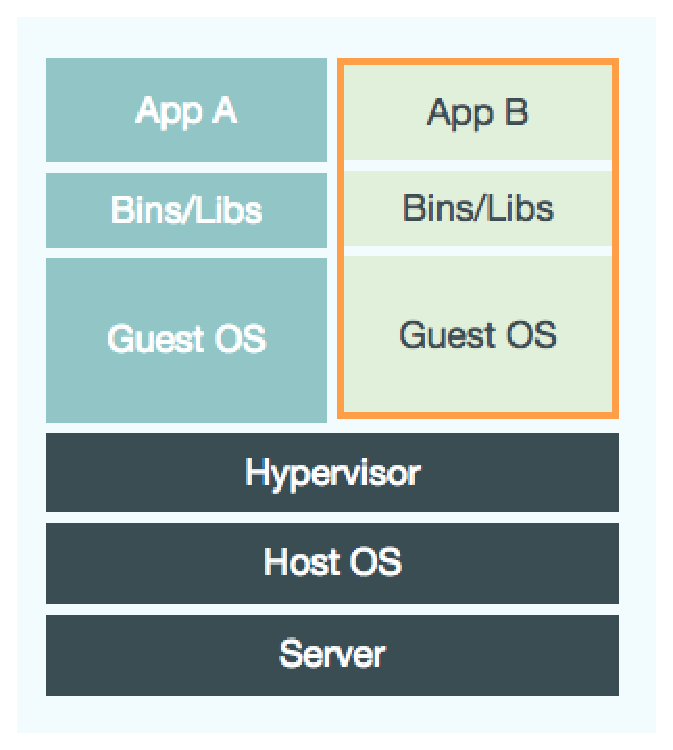
\includegraphics[width=1.8in]{virtual-machine.eps}}
		\subfigure[Docker]{\label{fig:docker}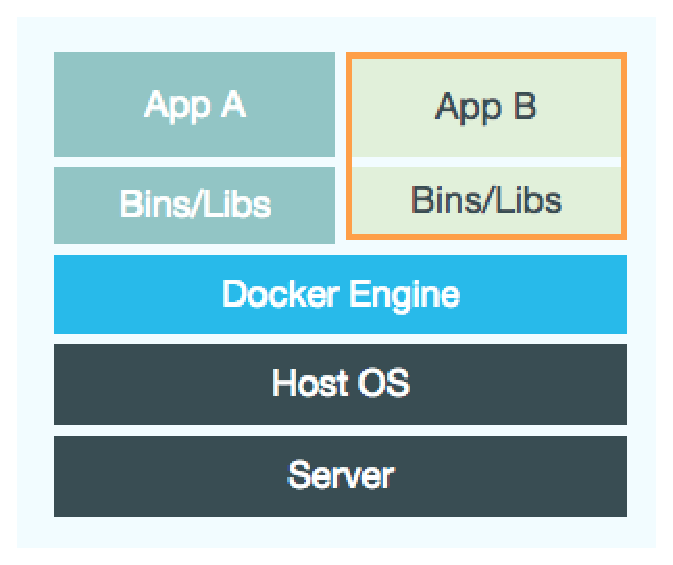
\includegraphics[width=1.8in]{docker.eps}}
		\caption{Virutal Machines V.s. Docker \cite {docker}}
		\label{fig:docker}
\end{figure}

Makahiki could utilize the Docker technology to provide a pre-configured docker container. An organization could just download this container and deploy to any cloud infrastructure they prefer with minimum installation or configuration effort. Once deployed, the organization can take advantage of the cloud infrastructure to dynamically manage the computing resources for the Makahiki game instance.

\subsection{Enhancement to Makahiki framework}
Lastly, Makahiki framework needs continuous enhancement. Some of the enhancement projects for Makahiki that we believe would be interesting and useful for the framework include:

\subsubsection{Real-time player awareness}
Currently it is not possible in Makahiki to know who is currently online and playing the game. Creating this awareness opens up new social gaming opportunities (performing tasks together), new opportunities for communication (chat windows), and potentially entirely new games (play against another online player). 

The goal of this enhancement is to extend the framework with a general purpose API that provides the identities of those who are online, and then the development of one or more user interface enhancements to exploit this capability.

\subsubsection{Deep Facebook integration}
Makahiki currently supports a ``shallow'' form of Facebook integration: you can request that your Facebook photo be used as your Makahiki profile picture, and you are given an opportunity to post to Facebook when the system notifies you of an accomplishment. 

One way to enhance the use of Facebook is to deepen the connection between user Facebook pages and their game play. This might involve more automated forms of notification (i.e. the same way ``Spotify'' playlists are posted to your Facebook wall), or ways in which your activities on Facebook could impact on your Makahiki challenge status. For example, posting a sustainability video to Facebook, or liking a Sustainability organization could earn you points. 

A different type of enhancement is to allow challenge designers to specify a Facebook page as the official Challenge Facebook information portal, and have the system automatically post information to that Facebook page as the challenge progresses.

\subsubsection{Customization of game analytics page}
\label{sec:future-game-manage}
Makahiki provides a one-page game analytics information for game designers and managers to monitor the game and get insights into the current status of a running game. The page currently crams 19 analytics widgets into one page, demanding a very large screen real estate to view the information in whole or the need of frequent scrolling. 

One enhancement is to provide admin users an additional interface to customize the appearance of the analytic widgets where they can choose which widget to appear. The individual widget could also support two types of appearance, one has larger display which provides full information and one has smaller display which provides minimum essential information. 

\subsubsection{Action Library Management System}
Makahiki currently ships with over 100 possible  ``actions'' already developed for the Smart Grid Game. However, the current implementation suffers from a number of problems:

There is no convenient way to display and peruse the current set of actions. This has led to a duplicate representation of the smart grid game, implemented using a Google Docs spreadsheet linked to Google Sites pages. This approach has a lot of problems: it duplicates content, it does not provide a way to edit or manage content, it is already out of date.

The content is intimately tied to the Smart Grid Game implementation. The SGG is just one of many ways that the sustainability content could be presented to players. By separating ``content'' from the ``presentation'', more games can be developed using this content. We could enhance Makahiki to provide a ``content management system'' for ``actions'', which could involve the following changes to the current Makahiki system:
\begin{itemize}
\item Library actions are created, view, and edit via a separate admin interface which is defined for the content authoring role
\item An editor is provided to create action content and preview it in a formatted manner.
\item Library actions can be ``instantiated'' into the Smart Grid Game. 
\item Library content can be exported and imported into systems in order to support sharing. 
\item A public repository can be provided on GitHub. The format could be JSON.
\end{itemize}

